%\documentclass[12pt]{article}
\documentclass[12pt, reqno]{article}
\usepackage[utf8]{inputenc}
\usepackage{amsthm, amsmath, amssymb, tikz, bm,diffcoeff}
\usepackage{verbatim}
%\usepackage{titlesec}
\usepackage{graphicx}
\usepackage[linesnumbered,ruled,vlined]{algorithm2e}
\usepackage{float}
\usepackage{derivative}
\usepackage{mathtools}
\usepackage{CJK} 
\usepackage{xifthen}
\usepackage{bbm}
\usepackage[colorlinks=true,
linkcolor=blue,citecolor=blue,
urlcolor=blue]{hyperref}
\usetikzlibrary{arrows,decorations.markings}
\usepackage[margin=1.0in]{geometry}
\usepackage{extarrows}
%\usepackage{ulem}

\usepackage[shortlabels]{enumitem}
\usepackage{todonotes}
\usetikzlibrary{calc,shapes, backgrounds}
\allowdisplaybreaks

\newtheorem{lemma}{Lemma}
\newtheorem{theorem}{Theorem}
%\newtheorem{corollary}{Corollary}
%\newtheorem{definition}{Definition}
\newtheorem{claim}{Claim}
\newtheorem{remark}{Remark}
\newtheorem{conjecture}{Conjecture}
\newtheorem{proposition}{Proposition}
\newtheorem{example}{Example}
\usepackage{tikz}

\newtheorem{cor}%[theorem]
{Corollary}

\newtheorem{defn}%[theorem]
{Definition}
\DeclareMathOperator{\ord}{ord}
\DeclareMathOperator{\lcm}{lcm}
\usepackage{mathtools}
\newcommand{\tb}{\textbf}
\newcommand{\R}{\mathbb{R}}
\newcommand{\II}{\mathcal{I}}
\newcommand{\tl}{\textsl}
\newcommand{\nf}{\normalfont}
\newcommand{\nd}{\noindent}
\newcommand{\mc}{\mathcal}
\newcommand{\mb}{\mathbb}
\DeclareMathOperator*{\esssup}{ess\,sup}
\DeclareMathOperator*{\essinf}{ess\,inf}
\DeclareMathOperator*{\argmax}{arg\,max}
\DeclareMathOperator*{\argmin}{arg\,min}
\usetikzlibrary{shapes,backgrounds}
\usepackage{verbatim}
\makeatother
\usepackage[inline]{asymptote}
\usepackage{extarrows}
\usepackage{hyperref}
\hypersetup{
    colorlinks,
    citecolor=black,
    filecolor=black,
    linkcolor=black,
    urlcolor=black
}

\title{Combinatorial Courant-Fischer-Weyl Minimax Principle on %Characterizations of 
Cheeger $k$-constants of Weighted Forests}
\author{Zijun Meng\thanks{Department of Mathematics, The Chinese University of Hong Kong,
Hong Kong, China. Email address: 1155194127@link.cuhk.edu.hk} \and Dong Zhang\thanks{School of Mathematical Sciences, Peking University,
100871 Beijing, China. Email address: dongzhang@math.pku.edu.cn}}

\date{}
\setlength {\marginparwidth }{2cm} 

\begin{document}

\maketitle

\begin{abstract}
We establish novel max-min and minimax characterizations of Cheeger $k$-constants in weighted forests, thereby providing the first combinatorial analogue of the Courant-\\Fischer-Weyl minimax principle. As for applications, we prove that the forest 1-Laplacian variational eigenvalues are independent of the choice of typical indexes; we propose a refined higher order Cheeger inequality involving numbers of loops of graphs and $p$-Laplacian eigenvalues; %this also implies 
and we present a combinatorial proof for the equality $h_k=\lambda_k(\Delta_1)$ which connects the 1-Laplacian variational eigenvalues and the multiway Cheeger constants. 
\end{abstract}
\tableofcontents

\section{Introduction}
The Cheeger $k$-constant is omnipresent in mathematics, it appears in different names in different fields, such as the \emph{higher isoperimetric numbers} (Daneshgar-Hajiabolhassan-Javadi, 2010, \cite{Daneshgar-Hajiabolhassan-Javadi}) and the \emph{$k$-way isoperimetric constant} (Mimura, 2016, \cite{Mimura}) in graph theory, the \emph{$k$-th Cheeger constant} (Bobkov-Parini, 2018, \cite{Bobkov-Parini}) for Euclidean spaces, and the \emph{connectivity spectrum} (Hassannezhad-Miclo, 2020, \cite{Hassannezhad-Miclo}) for Riemannian manifolds. %The Cheeger $k$-constant also has important connections with inequalities involving the $k$-th smallest eigenvalue of the Laplacian in the aforementioned fields \cite{Lee-Gharan-Trevisan,Hassannezhad-Miclo}.

The core contribution of the Cheeger k-constant lies in the fundamental inequality involving the Laplacian spectrum, and the connection to multi-partitioning and clustering problems in the aforementioned fields \cite{Lee-Gharan-Trevisan,Hassannezhad-Miclo}. Moreover, many of these results have been extended to the case of nonlinear eigenproblems \cite{Bungert}, particularly those of the $p$-Laplacian type \cite{Tudisco,Keller}.  %The Cheeger $k$-constant is also important in its own right.

In view its importance, we establish several max-min and min-max reformulations of multiway Cheeger constants of forests. These reformulations can be viewed as combinatorial analogues of the Courant-Fischer-Weyl minimax principle (see, for instance, Corollary III.1.2 of \cite{Bhatia}). We also provide two novel applications:
\begin{itemize}
\item Based on these reformulations, we first prove that several different types of min-max eigenvalues of the forest 1-Laplacian coincide. In fact, different types of min-max eigenvalues are defined using different indexes. A fundamental problem asks whether these min-max eigenvalues are independent of the choice of admissible indexes. We actually get an affirmative answer to this question for 1-Laplacians of forests. 
\item These max-min reformulations directly yield a rigorous proof of the 1-Laplacian Cheeger identity $\lambda_k(\Delta_1)=h_k$ for forests, which is in fact the first combinatorial proof. Combining this fact with previous results on the monotonicity of $p$-Laplacian eigenvalues, a refined multi-way Cheeger inequality for forests is established by using graph $p$-Laplacian instead of the normalized graph Laplacian. 
\end{itemize}

\subsection{%Known Results on 
Higher Order Cheeger Inequalities}
A \emph{(finite, undirected) weighted graph} $G$ is a quadruple $(V,E,\mu,w)$ with a \emph{vertex set} $V=\{1,\cdots,n\}$, an \emph{edge set} \[E\subseteq\{\{u,v\}:u\ne v\text{ in }V\},\] a \emph{vertex weight} $\mu:V\to \mathbb{R}^+$, and an \emph{edge weight} $w:E\to \R^+$. For simplicity, we use $w_{uv}$ and $\mu_v$ to denote $w(\{u,v\})$ and $\mu(v)$, respectively. 

Fix a weighted graph $G=(V,E,\mu,w)$. For any subset $A\subseteq V$ of vertices, define the \emph{boundary} $\partial A$ of $A$ by \[\partial A:=\{\{u,v\}\in E\colon u\in A, v\not\in A\}.\] Define the \emph{Cheeger $k$-constant} of $G$ by \[h_k(G):=\min_{\text{subpartitions }(A_1,\dots,A_k)\text{ of }V}~\max_{1\le i\le k}\phi(A_i),\] where \[\phi(A_i):=\phi_{\mu,w}(A_i):=\frac{w(\partial A)}{\mu(A)}:=\frac{\sum\limits_{\{u,v\}\in\partial A}w_{uv}}{\sum\limits_{v\in A}\mu_v}\] is the \textsl{expansion} (Lee-Oveis Gharan-Trevisan, \cite{Lee-Gharan-Trevisan}) of $A_i$, and by $(A_1,\dots,A_k)$ being a \emph{subpartition} of $V$ we mean that $A_i$ are pairwise disjoint nonempty subsets of $V$. 

Let $\lambda_{k}(\Delta_p)$ denote the $k$-th min-max eigenvalue of the graph $p$-Laplacian $\Delta_p$, where the relevant concepts and terminology are detailed in Section \ref{sec:minmax-eigen-1-Lap}. When $p=2$, $\Delta_2$ is called the \emph{(normalized) graph Laplacian}, and $\lambda_{k}(\Delta_2)$ is the $k$-th smallest eigenvalue of $\Delta_2$.  
We briefly list some known results on higher order Cheeger inequalities: 
\begin{itemize}
\item 
Lee-Oveis Gharan-Trevisan \cite{Lee-Gharan-Trevisan}: 
There exists a universal constant $C>0$ such that
$$\frac{1}{Ck^4}h_k(G)^2\le\lambda_k(\Delta_2)\le2h_k(G).$$

Note that the factor $\frac{1}{Ck^4}$ in the lower bound \textbf{depends on $k$}.
\item
Tudisco-Hein \cite{Tudisco}: For $p>1$, let $x$ be an eigenvector corresponding to the eigenvalue $\lambda_k(\Delta_p)$, and assume that $x$ has $m$ strong nodal domains. Then, $$ \frac{2^{p-1}}{p^p}h_m(G)^p\le\lambda_k(\Delta_p)\le 2^{p-1}h_k(G).$$

Here, the subscript $m$ of $h_m(G)^p$ in the lower bound \textbf{depends on the nodal domains of an eigenvector}. 
\item
Daneshgar-Javadi-Miclo \cite{Daneshgar,Miclo}: For any simple tree, 
$$\frac{1}{2}h_k(G)^2\le \lambda_{k}(\Delta_2)\le 2 h_k(G).$$

%The lower bound $\frac12h_k^2$ is sharp, but the inequality only works for the \textbf{Laplacian of forests}. 
\item
Deidda-Putti-Tudisco \cite{Deidda}: For any weighted tree, $$\lambda_{k}(\Delta_1)= h_k(G).$$ 

%However, the authors claimed this equality \textbf{without a rigorous proof}. 
\end{itemize}
Since the Cheeger $k$-constant $h_k(G)$ is defined via the minimax process, and $\lambda_{k}(\Delta_2)$ possesses a minimax representation according to the Courant-Fischer-Weyl theorem, a thorough examination of the minimax principle may deepen our understanding of these higher order Cheeger inequalities. This will lead to the discussion in subsequent sections.

\subsection{Minimax Principle}
There are some fundamental‌ equalities in the form of ``min-max = max-min'', such as the von Neumann minimax theorem for convex-concave functions \cite{Rockafellar} and the Courant-Fischer-Weyl minimax principle on the Rayleigh quotient \cite{Bhatia}. 
These capture very important information of the objective function, for example, von Neumann minimax theorem reveals the saddle data of a convex-concave function, while Courant-Fischer-Weyl theorem establishes minimax representation of eigenvalues of a self-adjoint operator. Since this paper focuses on min-max eigenvalues, we recall the Courant-Fischer-Weyl minimax principle as follows.

\begin{itemize}
\item For any symmetric matrix $\mathbf{A}\in \mathbb{R}^{n\times n}$, the $k$-th smallest eigenvalue $\lambda_k(\mathbf{A})$ can be written as 
$$ \lambda_k(\mathbf{A})=\min_{\substack{\text{linear subspaces }X\text{ of }\mathbb R^n\\\dim X\ge k}}~\max_{x\in X\setminus\{0\}} \frac{x^\top \mathbf{A} x}{x^\top x} = \max_{\substack{\text{linear subspaces }X\text{ of }\mathbb R^n\\\dim X\ge n-k+1}}~\min_{x\in X\setminus\{0\}} \frac{x^\top \mathbf{A} x}{x^\top x}.$$
\end{itemize}

It is worth noting that von Neumann minimax theorem involves duality which is commonly used in optimization, and thus many different analogues and generalizations have been obtained, e.g., there is a famous combinatorial version called the max-flow min-cut theorem. However, to the best of our knowledge, no combinatorial analogues of the Courant-Fischer-Weyl minimax principle had been proposed prior to our paper. 
Actually, if we focus solely on the ``min-max = max-min'' equality %\eqref{eq:minmax=maxmin-Courant} itself, 
\begin{equation}\label{eq:minmax=maxmin-Courant}
\min_{\substack{\text{linear subspaces }X\text{ of }\mathbb R^n\\\dim X= k}}~\max_{x\in X\setminus\{0\}} \frac{x^\top \mathbf{A} x}{x^\top x} = \max_{\substack{\text{linear subspaces }X\text{ of }\mathbb R^n\\\dim X= n-k+1}}~\min_{x\in X\setminus\{0\}} \frac{x^\top \mathbf{A} x}{x^\top x},   
\end{equation}
it would be surprising if \eqref{eq:minmax=maxmin-Courant} has no generalizations. %generalized forms.

This paper gives the first combinatorial and nonlinear analogues for the Courant-Fischer-Weyl minimax principle shown in terms of both Cheeger k-constant and k-th minimax $L^1$-Rayleigh quotient of forests. Specifically, we prove:
\begin{theorem}[combinatorial Courant-Fischer-Weyl minimax principle]\label{thm:CombinatorialCourant-Fischer}
For any forest $G=(V,E,\mu,w)$, we have \[\min_{\mathrm{subpartitions~}(A_1,\dots,A_{k})\mathrm{~of~}V}~~\max_{B\in \mathcal{U}(A_1,\cdots,A_{k})}\phi(B)=\max_{\mathrm{subpartitions~}(A_1,\dots,A_{n-k+1})\mathrm{~of~}V}~~\min_{B\in \mathcal{U}(A_1,\cdots,A_{n-k+1})}\phi(B),\]
where \[\mathcal{U}(A_1,\cdots,A_k)=\{A_{i_1}\cup\cdots\cup A_{i_q}:1\le i_1<\cdots<i_q\le k,\,1\le q\le k\}\] denotes the union-closed family generated by the subpartition $(A_1,\dots,A_{k})$ of $V$.
\end{theorem}

This form can be viewed as a combinatorial analog of the minimax principle on real symmetric matrices. 
It is known that \eqref{eq:minmax=maxmin-Courant} implies the Courant-Fischer-Weyl minimax principle for graph Laplacian:
\begin{equation}\label{eq:classical-minmax-Lap}
\min_{\substack{\text{linear subspaces }X\text{ of }\mathbb R^n\\\dim X= k}}~\max_{x\in X\setminus\{0\}} \frac{\sum\limits_{u\sim v}w_{uv}(x_u-x_v)^2}{\sum\limits_v\mu_vx_v^2} = \max_{\substack{\text{linear subspaces }X\text{ of }\mathbb R^n\\\dim X= n-k+1}}~\min_{x\in X\setminus\{0\}} \frac{\sum\limits_{u\sim v}w_{uv}(x_u-x_v)^2}{\sum\limits_v\mu_vx_v^2},
\end{equation}
where we write $u\sim v$ to mean $\{u,v\}$ is an edge. This minimax principle characterizes the $k$-th eigenvalue  $\lambda_k(\Delta_2)$ of the linear Laplacian on graphs. We propose a nonlinear analog of \eqref{eq:classical-minmax-Lap} as follows:
\begin{theorem}[nonlinear Courant-Fischer-Weyl minimax principle]\label{thm:nonlinearCourant-Fischer}
For any forest, 
\begin{align*}\min_{\substack{\mathrm{linear~subspaces~}X\mathrm{~of~}\mathbb R^n\\\dim X= k}}~\max_{x\in X\setminus\{0\}} \frac{\sum\limits_{u\sim v}w_{uv}|x_u-x_v|}{\sum\limits_v\mu_v|x_v|} = \max_{\substack{\mathrm{linear~subspaces~}X\mathrm{~of~}\mathbb R^n\\\dim X= n-k+1}}~\min_{x\in X\setminus\{0\}} \frac{\sum\limits_{u\sim v}w_{uv}|x_u-x_v|}{\sum\limits_v\mu_v|x_v|}
\end{align*}
\end{theorem}

It is noteworthy that both equalities in Theorem \ref{thm:CombinatorialCourant-Fischer} and Theorem \ref{thm:nonlinearCourant-Fischer} are equal to $h_k(G)$ when $G$ is a forest. 

These results are fascinating because equalities of the ``min-max = max-min'' form rarely arise in nonlinear or combinatorial situations. For example, in the field of nonlinear eigenvalue problems, there are many conjectures and open problems on ``min-max = max-min''  equalities \cite{Diening}. 

\section{Main Results}
To express results more concisely, we shall adopt some notation and conventions. 

Let \[\mathcal{P}_k(V):=\{(A_1,\dots,A_{k}):~\varnothing\ne A_i\subseteq V,\,A_i\cap A_j=\varnothing\,\forall i\ne j\}\] be the set of all subpartitions of $V$ with $k$ subsets. 

We have the following elementary observation:
\begin{proposition}\label{prop:unioninv}
%It can be verified that 
For any weighted graph $G=(V,E,\mu,w)$,
$$h_k(G):=\min_{(A_1,\dots,A_{k})\in \mathcal{P}_k(V)}~\max_{1\le i\le k}\phi(A_i)=\min_{(A_1,\dots,A_{k})\in \mathcal{P}_k(V)}~\max_{B\in \mathcal{U}(A_1,\cdots,A_{k})}\phi(B)$$
where \[\mathcal{U}(A_1,\cdots,A_k):=\{A_{i_1}\cup\cdots\cup A_{i_q}:1\le i_1<\cdots<i_q\le k,\,1\le q\le k\}\] stands for the union closed family generated by the $k$-tuple of sets $(A_1,\cdots,A_k)$. 
\end{proposition}
For any weighted graph $G=(V,E,\mu,w)$ with $n$ vertices, let 
$$\ell_k(G):=\max_{(A_1,\dots,A_{n-k+1})\in \mathcal{P}_{n-k+1}(V)}~\min_{B\in \mathcal{U}(A_1,\cdots,A_{n-k+1})}\phi(B)$$
be the $k$-th max-min Cheeger constant, and let $$\underline{\ell_k}(G) :=\max_{A\subseteq V,~|A|=n-k+1}h(A)$$ be the $k$-th Dirichlet Cheeger constant \cite{DTZ}, where \[h(A):=\min_{B\subseteq A}\phi(B)\] 
denotes the Cheeger constant of $A$ with respect to $G$. 
%Then, for any graph, we can establish the inequality $h_k\ge \ell_k\ge \underline{\ell_k} $. 

%We can actually show that $h_k=\ell_k=\underline{\ell_k} $ hold for forests, which derives the following minimax equality for forests:

We adopt a novel way, namely, by removing vertices from a subpartition of some suitably chosen subclass of subpartitions minimizing the maximum $\phi$-value, to prove our following main result of an alternate max-min characterization of the Cheeger $k$-constant of weighted forests:
\begin{theorem}\label{thm:h_k=H_k}
For any weighted graph $\tilde G=(\tilde V,\tilde E,\tilde\mu,\tilde w)$ with $n$ vertices, for any $k\in\{1,2,\cdots,n\}$, we have \[h_k(\tilde G)\ge \ell_k(\tilde G)\ge \underline{\ell_k}(\tilde G).\] 
For any weighted forest $G=(V,E,\mu,w)$ with $n$ vertices, we must have \[h_k(G)= \ell_k(G)= \underline{\ell_k}(G).\]
\end{theorem}
It is evident that the equality $h_k(G)= \ell_k(G)$ concerning forests in the aforementioned theorem is precisely the combinatorial Courant-Fischer-Weyl minimax principle we described in the introduction (see Theorem \ref{thm:CombinatorialCourant-Fischer}).

We present a generalization of {Theorem \ref{thm:h_k=H_k}} as follows.
\begin{theorem}\label{thm:cycle-number-inequ}
For any weighted graph $\tilde G=(\tilde V,\tilde E,\tilde\mu,\tilde w)$,  \[h_k(\tilde G)\ge \ell_k(\tilde G)\ge \underline{\ell_k}(\tilde G)\ge h_{k-\beta}(\tilde G),\] where $\beta:=|\tilde E|-|\tilde V|+c$ is the total number of independent loops of $\tilde G$, and $c$ is the number of connected components of $\tilde G$. 
\end{theorem}

%\section{Applications}
\subsection{Applications on min-max eigenvalues of Graph 1-Laplacian of Forests}\label{sec:minmax-eigen-1-Lap}
In the study of the $p$-Laplacian eigenvalue problem \cite{BH25,Burger,Drutu,Fazeny,HN25,Keller,LMR}, at least three sequences of eigenvalues have been introduced over the years. All of them are obtained by a \emph{minimax} procedure:
\begin{equation}\label{eq:continuous}
\lambda_k^{\mathrm{ind}}(\Delta_p):=\inf_{\substack{S\text{ origin-symmetric, compact}\\\mathrm{ind}(S)\ge k}}~\sup_{f\in S}\frac{\int_\Omega|\nabla f(z)|^pdz}{\int_\Omega|f(z)|^pdz}
\end{equation}
where $\mathrm{ind}(\cdot)$ is an admissible index for origin-symmetric compact subsets of the Sobolev space $H_0^1(\Omega)$. There are three admissible indexes commonly used for $p$-Laplacian:
\begin{itemize}
\item Krasnoselskii genus: The \emph{Krasnoselskii genus} of an origin-symmetric compact set $S$ is defined by $$\gamma(S):=\min\{k\in\mathbb{Z}^+:\exists\text{ odd continuous }\varphi:S\to \mathbb{R}^k\setminus\{0\}\}.$$ 
See \cite{Coffman} for details.
\item  Conner-Floyd index: The \emph{Conner-Floyd index} $\gamma^+$ of an origin-symmetric compact set $S$ is defined by $$\gamma^+(S):=\min\{k\in\mathbb{Z}^+:\exists\text{ odd continuous }\varphi:\mathbb{S}^{k-1}\to S\setminus\{0\}\},$$ 
where $\mathbb{S}^{k-1}$ stands for the unit sphere of $\mathbb{R}^k$. 
The min-max eigenvalues of $p$-Laplacian using $\mathrm{ind}=\gamma^+$ are called the Drabek-Robinson eigenvalues \cite{Drabek}.
\item Yang index: This index, denoted by $\textrm{Y-ind}(\cdot)$, is defined via homology information \cite{Yang}. We will not write down the definition explicitly, but interested readers may refer to \cite{Perera}.
\end{itemize}

The above three indices possess some common properties, which prompts us to introduce the following definition.

\begin{defn}[admissible index]
Let $\mathcal{S}$ be the set of all origin-symmetric compact subsets. 
An index $\mathrm{ind}:\mathcal{S}\to \mathbb{Z}_{\ge0}$ is \emph{admissible} if it satisfies the following properties:
\begin{itemize}
\item[(1)] %For any unit sphere of dimension 
$\mathrm{ind}(\mathbb{S}^{k-1})=k$, where $k=1,2,\cdots$
\item[(2)] monotonicity: If $A\subseteq A'$, then $$\mathrm{ind}(S)\le \mathrm{ind}(S').$$
\item[(3)] continuity: For any $S$, there exists a closed neighborhood $U$ of $S$ such that $$\mathrm{ind}(U)= \mathrm{ind}(S).$$
\item[(4)] nondecreasing under odd continuous map: For any odd continuous map $\eta$, $$\mathrm{ind}(S)\le  \mathrm{ind}(\eta(S)).$$
\end{itemize}
\end{defn}

By the standard approach in defining variational min-max eigenvalues of $\Delta_p$, we state that for every $k$, $\lambda_k^{\mathrm{ind}}(\Delta_p)$ defined with an admissible index must be an eigenvalue of $\Delta_p$ (see \cite{DTZ,Zhang}). 

It is known that $\lambda_1^{\gamma}(\Delta_p)= \lambda_1^{\gamma^+}(\Delta_p)$, $\lambda_2^{\gamma}(\Delta_p)= \lambda_2^{\gamma^+}(\Delta_p)$ and $\lambda_k^{\gamma}(\Delta_p)\le \lambda_k^{\gamma^+}(\Delta_p)$ for general $k$. However, the fundamental question of whether the general equality $\lambda_k^{\gamma}(\Delta_p)= \lambda_k^{\gamma^+}(\Delta_p)$ holds for every $k$ remains unresolved. For details, we refer to the open problem proposed by Luigi De Pascale in the 2013 Oberwolfach workshop \cite{Diening}.

In discrete settings, similar problems remain unsolved for the graph $p$-Laplacian. Let 
\begin{equation}\label{eq:discrete}
\lambda_k^{\mathrm{ind}}(\Delta_p):=\inf_{\substack{S\text{ origin-symmetric, compact}\\\mathrm{ind}(S)\ge k}}~\max_{x\in S}\frac{\sum\limits_{u\sim v}w_{uv}|x_u-x_v|^p}{\sum\limits_v\mu_v|x_v|^p} 
\end{equation}
be the min-max eigenvalue of $\Delta_p$ on a graph $G=(V,E,\mu,w)$, and let
\begin{equation}\label{eq:discrete/maxmin}
\underline{\lambda_k^{\mathrm{ind}}}(\Delta_p):=\sup_{\substack{S\text{ origin-symmetric, compact}\\\mathrm{ind}(S)\ge k}}~\min_{x\in S}\frac{\sum\limits_{u\sim v}w_{uv}|x_u-x_v|^p}{\sum\limits_v\mu_v|x_v|^p} 
\end{equation}
be the max-min eigenvalue of $\Delta_p$ on $G=(V,E,\mu,w)$ with $n$ vertices. 

As a direct corollary of Theorem \ref{thm:h_k=H_k}, we can give an affirmative answer to this question for 1-Laplacian of forests:

\begin{theorem}\label{thm:1-Lap=h}
Let $\Delta_1$ denote the 1-Laplacian of a forest $G$ with $n$ vertices. Then, for any admissible index, for any $k$, we have the equality
\begin{align*}
h_k(G)=\lambda_k^{\mathrm{ind}}(\Delta_1)=\underline{\lambda_k^{\mathrm{ind}}}(\Delta_1).%\sup_{S\text{ origin-symmetric, compact, }\mathrm{ind}(S)\ge n-k+1}\min_{x\in S}\frac{\sum\limits_{u\sim v}w_{uv}|x_u-x_v|}{\sum\limits_v\mu_v|x_v|}
\end{align*}
\end{theorem}

In particular, we have
\begin{cor}\label{cor:minmax-indepen-index}
Let $\Delta_1$ denote the 1-Laplacian of a forest. Then, for any $k$, 
$$ \lambda_k^{\gamma}(\Delta_1)=\lambda_k^{\gamma^+}(\Delta_1) =\lambda_k^{\textrm{Y-ind}}(\Delta_1).$$
\end{cor}

%$$ \lambda_k^{\mathrm{ind}}(\Delta_1)= \min_{\dim X= k}\max_{x\in X\setminus\{0\}} \frac{\sum\limits_{u\sim v}w_{uv}|x_u-x_v|}{\sum\limits_v\mu_v|x_v|} = \max_{\dim X= n-k+1}\min_{x\in X\setminus\{0\}} \frac{\sum\limits_{u\sim v}w_{uv}|x_u-x_v|}{\sum\limits_v\mu_v|x_v|}.$$
\begin{cor}[%proposed in 
\cite{Deidda-thesis,Deidda}]\label{cor:tree-1-Lap-h}
For any forest $G$, we have $$\lambda_{k}^\gamma(\Delta_1)= h_k(G).$$
\end{cor}

%Corollary \ref{cor:tree-1-Lap-h} first appeared in \cite{Deidda}. 
From Theorem \ref{thm:1-Lap=h}, we realize that Theorem \ref{thm:h_k=H_k} actually induces a combinatorial proof of Corollary \ref{cor:tree-1-Lap-h}. 

\subsection{Applications on Refined Multi-way Cheeger Inequalities%Our main contribution
}\label{sec:refined-Cheeger}

In this paper, we prove Theorems \ref{thm:h_k=H_k} and 
\ref{thm:cycle-number-inequ}, and combining with the known properties presented in Section \ref{sec:tools}, we improve the multi-way Cheeger inequality for forests and on graphs with a small total number of independent loops. We shall omit the superscript $\gamma$ in $\lambda_{k}^\gamma(\Delta_p)$ and write it as $\lambda_{k}(\Delta_p)$ instead. This is because most of the literature on graph $p$-Laplacians adopts this notation \cite{Deidda,LMR,Tudisco}. Furthermore, we assume that the vertex weights and the edge weights satisfy $\mu_v=\sum_{u\in V:u\sim v}w_{uv}$. Such an assumption is commonly employed because of the advantage that the factors in Cheeger's inequality are independent of the choice of edge weights.

Together with Corollary \ref{cor:tree-1-Lap-h} and a monotonicity property of the eigenvalues of graph $p$-Laplacian (c.f. \cite{Zhang}), we are able to establish the following multi-way  Cheeger inequality:

\begin{cor}\label{cor:tree-p-Lap}
For any weighted forest $G$ satisfying $\mu_v=\sum_{u\in V:u\sim v}w_{uv}$, $\forall v\in V$, for any $p\ge 1$, we have
$$\frac{2^{p-1}}{p^p}h_k(G)^p\le \lambda_{k}(\Delta_p)\le 2^{p-1} h_k(G).$$
\end{cor}

Corollary \ref{cor:tree-p-Lap} not only includes Corollary \ref{cor:tree-1-Lap-h} as a special case, but also refines the classical Cheeger inequality on trees by Miclo. 
We can rewrite the inequality in  {Corollary \ref{cor:tree-p-Lap}} as
$$
\swarrow\frac{1}{2^{p-1}}\lambda_k(\Delta_p)\le h_k(G)\le \frac p2 (2\lambda_k(\Delta_p))^{\frac1p}\nearrow.
$$
Then, by the increasing property of $\frac p2 (2\lambda_k(\Delta_p))^{\frac1p}$ with respect to $p\in[1,+\infty)$, and the decreasing property of $\frac{1}{2^{p-1}}\lambda_k(\Delta_p)$ with respect to $p\in[1,+\infty)$, the inequality becomes tight when $p$ tends to 1. 

Thanks to  {Theorem \ref{thm:cycle-number-inequ}}, {Corollary \ref{cor:tree-1-Lap-h}} can be generalized to apply to any graph with a small $\beta$.
\begin{theorem}\label{thm:beta}
For any weighted graph $G=(V,E,\mu,w)$, 
$$h_{k-\beta}(G) \le \lambda_{k}(\Delta_1)\le h_k(G),$$
where $\beta:=|E|-|V|+1$. %is the total number of independent loops of the graph. 
\end{theorem}

Similarly, we can generalize {Corollary \ref{cor:tree-p-Lap}} to the following formulation:
\begin{theorem}\label{thm:beta-p}
For any weighted graph $G=(V,E,\mu,w)$ satisfying $\mu_v=\sum_{u\in V:u\sim v}w_{uv}$, $\forall v\in V$, for any $p\ge 1$, we have 
$$\frac{2^{p-1}}{p^p}h_{k-\beta}(G)^p\le \lambda_{k}(\Delta_p)\le 2^{p-1} h_k(G).$$
\end{theorem}

Note that the subscript $k-\beta$ of the term $h_{k-\beta}$ does not depend on the nodal domain counts, and the factor $\frac{2^{p-1}}{p^p}$ in the lower bound is independent of both $k$ and graphs. This improves the main theorem in \cite{Tudisco}. 

A \emph{unicyclic graph} is a graph that has exactly one circuit. 
\begin{cor}\label{cor:unicyclic}
For any weighted unicyclic graph $G=(V,E,\mu,w)$ satisfying $\mu_v=\sum_{u\in V:u\sim v}w_{uv}$, $\forall v\in V$, we have $\frac{2^{p-1}}{p^p}h_{k-1}(G)\le \lambda_{k}(\Delta_p)\le 2^{p-1} h_k(G)$.   
\end{cor}
%Particularly, for any unicyclic graph,  $\beta=1$ and the inequality $\frac{2^{p-1}}{p^p}h_{k-1}(G)\le \lambda_{k}(\Delta_p)\le 2^{p-1} h_k(G)$ is actually sharp.

\section{Proofs}
This section is devoted to providing detailed proofs of all the theorems presented in this paper. Figure \ref{fig:placeholder} describes the logic flow between our results, rectangles indicate combinatorial results, ellipses indicate analytical results, white indicates auxiliary and less important results, grey indicates main results.

\tikzstyle{startstop} = [ellipse, rounded corners, minimum width=1cm, minimum height=1cm,text centered, draw=black, fill=white]
\tikzstyle{startstop2} = [ellipse, minimum width=1cm, minimum height=1cm,text centered, draw=black, fill=gray!10]
\tikzstyle{startstop3} = [rectangle, minimum width=1cm, minimum height=1cm,text centered, draw=black, fill=white]
\tikzstyle{startstop4} = [rectangle, minimum width=1cm, minimum height=1cm,text centered, draw=black, fill=gray!10]

\begin{figure}
    \centering
\begin{tikzpicture}[scale=1,node distance=3.9cm]
\node(L1)[startstop3]{Lemma \ref{lemma:basic-phi} };
\node(L2)[startstop3,below of=L1,yshift=1.5cm,xshift=-3.5cm]{Lemma \ref{lem:cheeger-set-disjoint}};  
\node(L3)[startstop3,below of=L1,yshift=2.6cm,xshift=0cm]{Lemma \ref{lem:pigeonhole}};  
\node(P1)[startstop3,below of=L1,yshift=-0.5cm,xshift=0cm]{Proposition \ref{prop:unioninv}};
\node(T3)[startstop4,right of=L2,yshift=0cm,xshift=3cm]{Theorem \ref{thm:h_k=H_k}};
\node(T4)[startstop4,below of=T3,yshift=-8cm,xshift=0cm]{Theorem \ref{thm:cycle-number-inequ}};
\node(T6)[startstop2,right of=T4,yshift=4cm,xshift=0cm]{Theorem \ref{thm:beta}};
\node(T1)[startstop4,below of=T3,yshift=-1.5cm,xshift=-1.5cm]{Theorem \ref{thm:CombinatorialCourant-Fischer}};
\node(T5)[startstop2,right of=T3,yshift=6cm,xshift=-3.8cm]{Theorem \ref{thm:1-Lap=h}};
\node(C2)[startstop,above of=T5,yshift=-2cm,xshift=4cm]{Corollary \ref{cor:tree-1-Lap-h}};
\node(C1)[startstop,left of=T5,yshift=0cm,xshift=0cm]{Corollary \ref{cor:minmax-indepen-index}};
\node(T2)[startstop2,right of=T3,yshift=2cm,xshift=-2cm]{Theorem \ref{thm:nonlinearCourant-Fischer}};
\node(L4)[startstop,above of=T5,yshift=-8cm,xshift=8cm]{Lemma \ref{lem:p-monotonicity}};
\node(C3)[startstop,above of=L4,yshift=0cm,xshift=0cm]{Corollary \ref{cor:tree-p-Lap}};
\node(L7)[startstop,below of=T5,yshift=2cm,xshift=3.5cm]{Lemma \ref{lem:general-graph-delta}};
\node(L6)[startstop,below of=L7,yshift=0cm,xshift=2cm]{Lemma \ref{lem:levelset}};
\node(L5)[startstop,above of=L7,yshift=-2cm,xshift=0cm]{Lemma \ref{lem:intersect}};
\node(T7)[startstop2,below of=L4,yshift=0cm,xshift=0cm]{Theorem \ref{thm:beta-p}};
\node(C4)[startstop,below of=T7,yshift=1cm,xshift=0cm]{Corollary \ref{cor:unicyclic}};
\draw[decoration={markings,mark=at position 1 with{\arrow[scale=2,>=stealth]{>}}},postaction={decorate}](P1) to%[out=140,in=40]
node[anchor=south]{ } (T3);
\draw[decoration={markings,mark=at position 1 with{\arrow[scale=2,>=stealth]{>}}},postaction={decorate}](L1) to%[out=165,in=275]  
node[anchor=north] { }(T3);
\draw[decoration={markings,mark=at position 1 with{\arrow[scale=2,>=stealth]{>}}},postaction={decorate}](L2) to%[out=165,in=275]  
node[anchor=north] { }(T3);
\draw[decoration={markings,mark=at position 1 with{\arrow[scale=2,>=stealth]{>}}},postaction={decorate}](L2) to%[out=165,in=275]  
node[anchor=north] { }(P1);
\draw[decoration={markings,mark=at position 1 with{\arrow[scale=2,>=stealth]{>}}},postaction={decorate}](L3) to%[out=165,in=275]  
node[anchor=north] { }(T3);
\draw[decoration={markings,mark=at position 1 with{\arrow[scale=2,>=stealth]{>}}},postaction={decorate}](L1) to%[out=210,in=75]  
node[anchor=north] { }(L2);
\draw[decoration={markings,mark=at position 1 with{\arrow[scale=2,>=stealth]{>}}},postaction={decorate}](T3) to%[out=235,in=45] 
node[anchor=north]{ } (T5);
\draw[decoration={markings,mark=at position 1 with{\arrow[scale=2,>=stealth]{>}}},postaction={decorate}](T3) to%[out=235,in=45] 
node[anchor=north]{ } (T4);
\draw[decoration={markings,mark=at position 1 with{\arrow[scale=2,>=stealth]{>}}},postaction={decorate}](T3) to%[out=235,in=45] 
node[anchor=north]{ } (T1);
\draw[decoration={markings,mark=at position 1 with{\arrow[scale=2,>=stealth]{>}}},postaction={decorate}](T4)to node[anchor=north]{ }(T6);
\draw[decoration={markings,mark=at position 1 with{\arrow[scale=2,>=stealth]{>}}},postaction={decorate}](T3) to node[anchor=north]{ }(T6);
\draw[decoration={markings,mark=at position 1 with{\arrow[scale=2,>=stealth]{>}}},postaction={decorate}](L7) to node[anchor=north]{ }(T6);
\draw[decoration={markings,mark=at position 1 with{\arrow[scale=2,>=stealth]{>}}},postaction={decorate}](L7) to node[anchor=north]{ }(T2);
\draw[decoration={markings,mark=at position 1 with{\arrow[scale=2,>=stealth]{>}}},postaction={decorate}](T3) to node[anchor=north]{ }(T2);
\draw[decoration={markings,mark=at position 1 with{\arrow[scale=2,>=stealth]{>}}},postaction={decorate}](T6) to node[anchor=north]{ }(T7);
\draw[decoration={markings,mark=at position 1 with{\arrow[scale=2,>=stealth]{>}}},postaction={decorate}](L4) to node[anchor=north]{ }(T7);
\draw[decoration={markings,mark=at position 1 with{\arrow[scale=2,>=stealth]{>}}},postaction={decorate}](L7) to node[anchor=north]{ }(T5);
\draw[decoration={markings,mark=at position 1 with{\arrow[scale=2,>=stealth]{>}}},postaction={decorate}](L5) to node[anchor=north]{ }(L7);
\draw[decoration={markings,mark=at position 1 with{\arrow[scale=2,>=stealth]{>}}},postaction={decorate}](L6) to node[anchor=north]{ }(L7);
\draw[decoration={markings,mark=at position 1 with{\arrow[scale=2,>=stealth]{>}}},postaction={decorate}](P1) to node[anchor=north]{ }(T1);
\draw[decoration={markings,mark=at position 1 with{\arrow[scale=2,>=stealth]{>}}},postaction={decorate}](T5) to node[anchor=north]{ }(C1);
\draw[decoration={markings,mark=at position 1 with{\arrow[scale=2,>=stealth]{>}}},postaction={decorate}](T5) to node[anchor=north]{ }(C2);
\draw[decoration={markings,mark=at position 1 with{\arrow[scale=2,>=stealth]{>}}},postaction={decorate}](C2) to node[anchor=north]{ }(C3);
\draw[decoration={markings,mark=at position 1 with{\arrow[scale=2,>=stealth]{>}}},postaction={decorate}](L4) to node[anchor=north]{ }(C3);
\draw[decoration={markings,mark=at position 1 with{\arrow[scale=2,>=stealth]{>}}},postaction={decorate}](L2) to node[anchor=north]{ }(T4);
\draw[decoration={markings,mark=at position 1 with{\arrow[scale=2,>=stealth]{>}}},postaction={decorate}](T7) to node[anchor=north]{ }(C4);
\end{tikzpicture}
    \caption{Logic Flow}
    \label{fig:placeholder}
\end{figure}

\subsection{Proofs of the Main Theorems (Combinatorial)}
For any two nonempty disjoint subsets $A$ and $B$ of $V$, define \[E(A,B):=\{\{u,v\}\in E:u\in A,v\in B\}\] to be the set of edges with one vertex in $A$ and the other in $B$. Two nonempty disjoint subsets $A$ and $B$ are said to be \emph{nonadjacent} if $E(A,B)=\varnothing$.

\begin{lemma}\label{lemma:basic-phi}
For any disjoint subsets $A$ and $B$ of $V$, we have $\phi(A\cup B)\le \max\left\{\phi(A),\phi(B)\right\}$. If we further assume that $E(A,B)=\varnothing$, then we have $$\min\left\{\phi(A),\phi(B)\right\} \le \phi(A\cup B)\le \max\left\{\phi(A),\phi(B)\right\}.$$
\end{lemma}

%\subsubsection{Proof of Lemma \ref{lemma:basic-phi}}
\begin{proof}[Proof of Lemma \ref{lemma:basic-phi}]
Let $a=w(\partial A)$, $b=\mu(A)$, $c=w(\partial B)$, $d=\mu(B)$. Then \[w(\partial(A\cup B))\le a+c\text{ and }\mu(A\cup B)=b+d,\] so $\phi(A\cup B)\le\frac{a+c}{b+d}$. Now suppose for the sake of contradiction that \[\frac ab<\frac{a+c}{b+d}\text{ and }\frac cd<\frac{a+c}{b+d},\] then summing up yields \[\frac{ad+bc}{bd}<\frac{a+c}{b+d}\iff ad^2+b^2c<0,\] which is a contradiction, so it follows that $\phi(A\cup B)\le\max\{\phi(A),\phi(B)\}$. If in addition $E(A,B)=\varnothing$, then $w(\partial(A\cup B))=a+c$ and $\phi(A\cup B)=\frac{a+c}{b+d}$, so the remaining inequality follows similarly.
\end{proof}

The next statement is a consequence of the preceding lemma.

\begin{lemma}\label{lem:cheeger-set-disjoint}
For any subpartition $(B_1,\cdots,B_k)$ of $V$, we have \[h(B_1\cup\cdots\cup B_k)\le \min\{h(B_1),\cdots,h(B_k)\}.\] If we further assume that $E(B_i,B_j)=\varnothing$ whenever $i\ne j$, then we have \[h(B_1\cup\cdots\cup B_k)=\min\{h(B_1),\cdots,h(B_k)\}.\]
\end{lemma}

%\subsubsection{Proof of Lemma \ref{lem:cheeger-set-disjoint}}
\begin{proof}[Proof of Lemma \ref{lem:cheeger-set-disjoint}]
Suppose $C\subseteq B_1\cup\dots\cup B_k$ is such that $\phi(C)=h(B_1\cup\dots\cup B_k)$, then we can assume that $C$ is connected, because otherwise we can replace $C$ by one of its connected components that possesses the minimum $\phi$-value without affecting the minimality by Lemma \ref{lemma:basic-phi}, so $C\subseteq B_j$ for some $1\le j\le k$. Thus, \[\phi(C)=h(B_j)=\min\{h(B_1),\dots,h(B_k)\},\] this concludes the proof.
\end{proof}

We note that the geometric versions of Lemmas \ref{lemma:basic-phi} and \ref{lem:cheeger-set-disjoint} are known \cite{Bobkov-Parini,Mazon}. 

\begin{lemma}\label{lem:pigeonhole}
Let $n$ be a positive integer. Suppose that \[(A_1,\dots,A_k)\text{ and }(B_1,\dots,B_{n-k+1})\] are subpartitions of $[n]:=\{1,\dots, n\}$, then there exists a nonempty subset $\{i_1,\dots,i_t\}$ of $[k]$ and a nonempty subset $\{j_1,\dots,j_s\}$ of $[n-k+1]$ such that \[A_{i_1}\cup\dots\cup A_{i_t}=B_{j_1}\cup\dots\cup B_{j_s}.\]
\end{lemma}

\begin{proof}[Proof of Lemma \ref{lem:pigeonhole}]
We apply strong induction on $n$. The base case $n=1$ is obvious. In general, if $(A_1,\dots,A_k)$ and $(B_1,\dots,B_{n-k+1})$ are partitions of $[n]$, then we are done. Otherwise, let \[C=\left(\bigcup_{1\le i\le k} A_i\right)\bigcap\left(\bigcup_{1\le j\le n-k+1} B_j\right),\] then we have $c:=|C|<n$. Note that at most $n-c$ subsets among the $A_i$'s and the $B_j$'s contain elements outside $C$. In other words, at least $c+1$ subsets contain only elements in $C$. Now we apply the induction hypothesis on $C$ and the two subpartitions formed by those at least $c+1$ subsets.
\end{proof}

\subsubsection{Proof of Proposition \ref{prop:unioninv}}
\begin{proof}
The proposition follows immediately from Lemma \ref{lem:cheeger-set-disjoint}, which implies that choosing from $\mathcal U(A_1,\dots,A_k)$ will not make it strictly larger than choosing from $\{A_1,\dots,A_k\}$.
\end{proof}

\subsubsection{Proof of Theorem \ref{thm:h_k=H_k}}
\begin{proof}
Due to its overwhelming length, we divide our proof into several steps.

\vspace{0.3cm}

\noindent\underline{Step 1. Setup.}
\newline\noindent For ease of presentation, we prove the case when $G$ is a weighted tree, whereas the proof for the general case of weighted forests is done by mimicking the following proof. Let \[S_1:=\argmin_{\mathcal A=(A_1,\dots,A_k)\in\mathcal{P}_k(V)}~\max_{1\le i\le k}\phi(A_i)\] be the set of all subpartitions that minimize the maximum $\phi$-value among the subsets. For reasons that will become clear later, we do not attempt to start working on a subpartition in $S_1$. Instead, we need more requirements on the subpartitions than that and furthur refine our desired class by letting \[S_2:=\argmin_{\mathcal A=(A_1,\dots,A_k)\in S_1}f(\mathcal A),\] where \[f(\mathcal A)=|\{1\le i\le k\colon\phi(A_i)=h_k\}|,\] be the set of all subpartitions in $S_1$ minimizing the number of subsets sharing the maximum $\phi$-value and \[S_3:=\argmin_{\mathcal A=(A_1,\dots,A_k)\in S_2}~\sum_{i=1}^k\mu(A_i)\] be the set of all subpartitions in $S_2$ that minimize the total weighted degree. Now, pick any subpartition $\mathcal A=(A_1,\dots,A_k)\in S_3$. By reordering if necessary, suppose that \[\phi(A_1)\le\dots\le\phi(A_k)=h_k\] without loss of generality.

\vspace{0.3cm}

\noindent\underline{Step 2. Achieving pairwise nonadjacency.}
\newline\noindent We prove that there exists $v_1\in A_1,\dots,v_{k-1}\in A_{k-1}$ such that \[A_1\setminus\{v_1\},\dots,A_{k-1}\setminus\{v_{k-1}\},V\setminus(A_1\cup\dots\cup A_{k-1})\] are pairwise nonadjacent in this step.

Indeed, since $\mathcal A=(A_1,\dots,A_k)\in S_3$, each $A_i$ is connected. (This is because otherwise, if some $A_j$ is not connected, then we write \[A_j=A_{j1}\cup\dots\cup A_{jm},\] where $A_{j1},\dots,A_{jm}$ are the $m$ connected components of $A_j$. Now, by Lemma \ref{lemma:basic-phi}, since \[E(A_{j1},A_{j2}\cup\dots\cup A_{jm})=\varnothing,\] we have \[\min\{\phi(A_{j1}),\phi(A_{j2}\cup\dots\cup A_{jm})\}\le\phi(A_j).\] If it happens that $\phi(A_{j1})>\phi(A_j)$, then we apply Lemma \ref{lemma:basic-phi} and the same procedure on \[A_{j2}\cup\dots\cup A_{jm}=A_{j2}\cup(A_{j3}\cup\dots\cup A_{jm}),\] and eventually we will obtain some $1\le p\le m$ such that $\phi(A_{jp})\le\phi(A_j)$. Now note that the subpartition \[\tilde{\mathcal A}=(A_1,\dots,A_{jp},\dots,A_k)\] is in $S_1$, since replacing by $A_j$ by $A_{jp}$ does not increase the maximum $\phi$-value. For this same reason, we can infer that $\tilde{\mathcal A}\in S_2$ as well. However, the total weighted degree of $\tilde{\mathcal A}$ is smaller than that of $\mathcal A$, which contradicts the assumption that $\mathcal A\in S_3$. Therefore, each $A_i$ is connected.) Now, recall that the graph $G$ we are working on is assumed to be a tree, so we can make the $k$ connected subsets $A_1,\dots,A_k$ pairwise nonadjacent by removing a vertex in each of some $k-1$ subsets. (See Figure \ref{fig:pairwisenonadj}).

\begin{comment}
\begin{figure}[h!]
\centering
\includegraphics[scale=0.15]{thm1.jpg}
\caption{Choosing $v_1,\dots,v_{k-1}$}
\end{figure}
\end{comment}

\begin{figure}
\centering
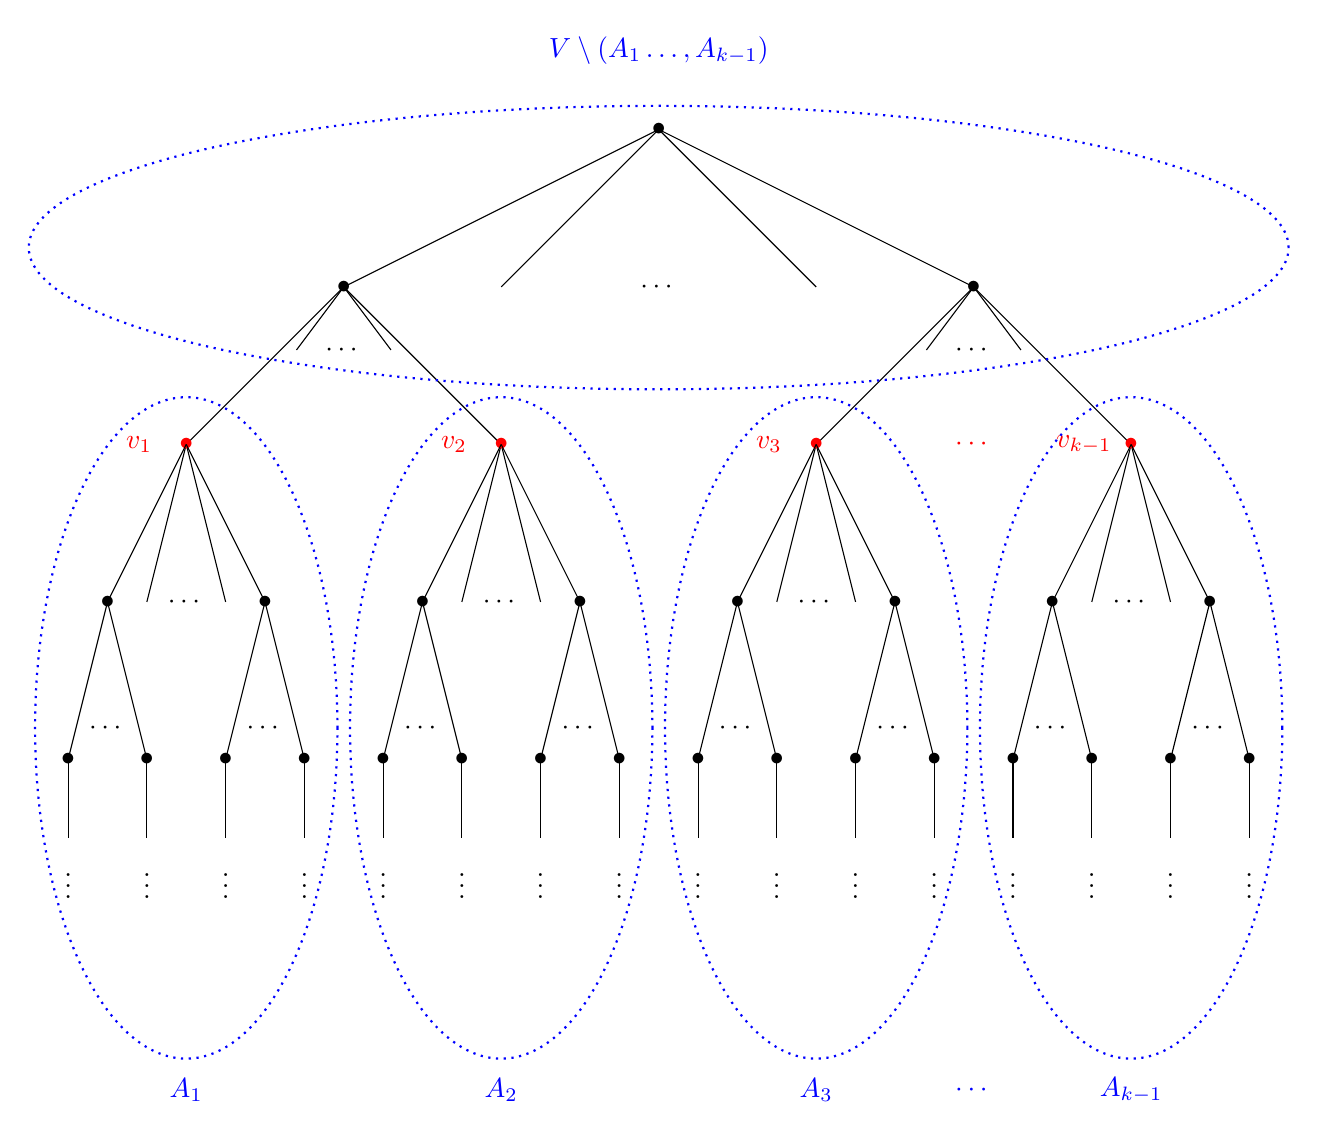
\begin{tikzpicture}[scale=2]
\draw (0,0)--(-2,-1)--(-3,-2);
\draw (0,0)--(-1,-1);
\draw (0,0)--(1,-1);
\draw (0,0)--(2,-1)--(3,-2);
\draw (2,-1)--(1.7,-1.4);
\draw (2,-1)--(2.3,-1.4);
\draw (-2,-1)--(-2.3,-1.4);
\draw (-2,-1)--(-1.7,-1.4);
\draw (-2,-1)--(-1,-2);
\draw (2,-1)--(1,-2);
\draw (-3,-2)--(-3.25,-3);
\draw (-3,-2)--(-2.75,-3);
\draw (-1,-2)--(-1.25,-3);
\draw (-1,-2)--(-0.75,-3);
\draw (1,-2)--(0.75,-3);
\draw (1,-2)--(1.25,-3);
\draw (3,-2)--(2.75,-3);
\draw (3,-2)--(3.25,-3);
\draw (-3.75,-4)--(-3.75,-4.5);
\draw (-3.25,-4)--(-3.25,-4.5);
\draw (-2.75,-4)--(-2.75,-4.5);
\draw (-2.25,-4)--(-2.25,-4.5);
\draw (-1.75,-4)--(-1.75,-4.5);
\draw (-1.25,-4)--(-1.25,-4.5);
\draw (-0.75,-4)--(-0.75,-4.5);
\draw (-0.25,-4)--(-0.25,-4.5);
\draw (0.25,-4)--(0.25,-4.5);
\draw (0.75,-4)--(0.75,-4.5);
\draw (1.25,-4)--(1.25,-4.5);
\draw (1.75,-4)--(1.75,-4.5);
\draw (2.25,-4)--(2.25,-4.5);
\draw (2.75,-4)--(2.75,-4.5);
\draw (3.25,-4)--(3.25,-4.5);
\draw (3.75,-4)--(3.75,-4.5);
\node (1) at (0,0) {$\bullet$};
\node (1) at (-2,-1) {$\bullet$};
\node (1) at (2,-1) {$\bullet$};
\node (1) at (2,-1.4) {$\cdots$};
\node (1) at (-2,-1.4) {$\cdots$};
\node (1) at (-3,-3) {$\cdots$};
\node (1) at (-1,-3) {$\cdots$};
\node (1) at (1,-3) {$\cdots$};
\node (1) at (3,-3) {$\cdots$};
\node (1) at (-3.5,-3.8) {$\cdots$};
\node (1) at (-2.5,-3.8) {$\cdots$};
\node (1) at (-1.5,-3.8) {$\cdots$};
\node (1) at (-0.5,-3.8) {$\cdots$};
\node (1) at (0.5,-3.8) {$\cdots$};
\node (1) at (1.5,-3.8) {$\cdots$};
\node (1) at (2.5,-3.8) {$\cdots$};
\node (1) at (3.5,-3.8) {$\cdots$};
\node (1) at (0,-1) {$\cdots$};
\node (1) at (-3.75,-4.75) {$\vdots$};
\node (1) at (-3.25,-4.75) {$\vdots$};
\node (1) at (-2.75,-4.75) {$\vdots$};
\node (1) at (-2.25,-4.75) {$\vdots$};
\node (1) at (-1.75,-4.75) {$\vdots$};
\node (1) at (-1.25,-4.75) {$\vdots$};
\node (1) at (-0.75,-4.75) {$\vdots$};
\node (1) at (-0.25,-4.75) {$\vdots$};
\node (1) at (0.25,-4.75) {$\vdots$};
\node (1) at (0.75,-4.75) {$\vdots$};
\node (1) at (1.25,-4.75) {$\vdots$};
\node (1) at (1.75,-4.75) {$\vdots$};
\node (1) at (2.25,-4.75) {$\vdots$};
\node (1) at (2.75,-4.75) {$\vdots$};
\node (1) at (3.25,-4.75) {$\vdots$};
\node (1) at (3.75,-4.75) {$\vdots$};
\node (1) at (2,-6.1) {\color{blue}$\cdots$};
\node (1) at (2,-2) {\color{red}$\cdots$};

\node (1) at (-3,-2) {\color{red}$\bullet$};
\node (v1) at (-3.3,-2) {\color{red}$v_1$};
\draw[blue,dotted,thick] (-3,-3.8)ellipse(0.96cm and 2.1cm);
\node (A1) at (-3,-6.1){\color{blue}$A_1$};
\draw (-3,-2)--(-3.5,-3)--(-3.25,-4);
\draw (-3.5,-3)--(-3.75,-4);
\draw (-2.25,-4)--(-2.5,-3)--(-2.75,-4);
\draw (-3,-2)--(-2.5,-3);
\node (1) at (-3.5,-3) {$\bullet$};
\node (1) at (-2.5,-3) {$\bullet$};
\node (1) at (-3.75,-4){$\bullet$};
\node (1) at (-3.25,-4){$\bullet$};
\node (1) at (-2.75,-4){$\bullet$};
\node (1) at (-2.25,-4){$\bullet$};

\node (v2) at (-1.3,-2) {\color{red}$v_2$};
\node (1) at (-1,-2) {\color{red}$\bullet$};
\draw[blue,dotted,thick] (-1,-3.8)ellipse(0.96cm and 2.1cm);
\node (A2) at (-1,-6.1){\color{blue}$A_2$};
\draw (-1,-2)--(-1.5,-3)--(-1.25,-4);
\draw (-1.5,-3)--(-1.75,-4);
\draw (-0.25,-4)--(-0.5,-3)--(-0.75,-4);
\draw (-1,-2)--(-0.5,-3);
\node (1) at (-1.5,-3) {$\bullet$};
\node (1) at (-0.5,-3) {$\bullet$};
\node (1) at (-1.75,-4){$\bullet$};
\node (1) at (-1.25,-4){$\bullet$};
\node (1) at (-0.75,-4){$\bullet$};
\node (1) at (-0.25,-4){$\bullet$};

\node (v3) at (0.7,-2) {\color{red}$v_3$};
\node (1) at (1,-2) {\color{red}$\bullet$};
\draw[blue,dotted,thick] (1,-3.8)ellipse(0.96cm and 2.1cm);
\node (A3) at (1,-6.1){\color{blue}$A_3$};
\draw (1,-2)--(0.5,-3)--(0.75,-4);
\draw (0.5,-3)--(0.25,-4);
\draw (1.75,-4)--(1.5,-3)--(1.25,-4);
\draw (1,-2)--(1.5,-3);
\node (1) at (0.5,-3) {$\bullet$};
\node (1) at (1.5,-3) {$\bullet$};
\node (1) at (0.25,-4){$\bullet$};
\node (1) at (0.75,-4){$\bullet$};
\node (1) at (1.25,-4){$\bullet$};
\node (1) at (1.75,-4){$\bullet$};

\node (v4) at (2.7,-2) {\color{red}$v_{k-1}$};
\node (1) at (3,-2) {\color{red}$\bullet$};
\draw[blue,dotted,thick] (3,-3.8)ellipse(0.96cm and 2.1cm);
\node (A4) at (3,-6.1){\color{blue}$A_{k-1}$};
\draw (3,-2)--(2.5,-3)--(2.75,-4);
\draw (2.5,-3)--(2.25,-4);
\draw (3.75,-4)--(3.5,-3)--(3.25,-4);
\draw (3,-2)--(3.5,-3);
\node (1) at (2.5,-3) {$\bullet$};
\node (1) at (3.5,-3) {$\bullet$};
\node (1) at (2.25,-4){$\bullet$};
\node (1) at (2.75,-4){$\bullet$};
\node (1) at (3.25,-4){$\bullet$};
\node (1) at (3.75,-4){$\bullet$};

\draw[blue,dotted,thick] (0,-0.75)ellipse(4cm and 0.9cm);
\node (V) at (0,0.5){\color{blue}$V\setminus(A_1\dots,A_{k-1})$};
\end{tikzpicture}
\caption{Choosing $v_1,\dots,v_{k-1}$.}
\label{fig:pairwisenonadj}
\end{figure}

\vspace{0.3cm}

\noindent\underline{Step 3. Showing $h(V\setminus(A_1\cup\dots\cup A_{k-1}))=h_k(G)$.}
\newline\noindent Firstly, note that we have \[h(V\setminus(A_1\cup\dots\cup A_{k-1}))\le h_k(G).\] Indeed, since \[A_k\subseteq V\setminus(A_1\cup\dots\cup A_{k-1}),\] we have \[h(V\setminus(A_1\cup\dots\cup A_{k-1}))=\min_{C\subseteq V\setminus(A_1\cup\dots\cup A_{k-1})}\phi(C)\le\phi(A_k)=h_k(G).\]

Next, for the sake of contradiction, we suppose that $h(V\setminus(A_1\cup\dots\cup A_{k-1}))<h_k(G)$. Then, by the definition of $h$, there is some $A_k'\subseteq V\setminus(A_1\cup\dots\cup A_{k-1})$ such that \[\phi(A_k')=h(V\setminus(A_1\cup\dots\cup A_{k-1}))<h_k(G).\] Then, we can replace $A_k$ by $A_k'$ and consider the subpartition \[\mathcal A':=(A_1',\dots,A_{k-1}',A_k'):=(A_1,\dots,A_{k-1},A_k'),\] where $A_i':=A_i$ for $1\le i\le k-1$. We divide into two cases:

\vspace{0.3cm}

\noindent\textsl{Case 1.} $\phi(A_{k-1})=\phi(A_k)=h_k(G)$.
\newline Then, $f(\mathcal A')=f(\mathcal A)-1<f(\mathcal A)$ contradicts the assumption that $\mathcal A\in S_3\subseteq S_2$.

\vspace{0.3cm}

\noindent\textsl{Case 2.} $\phi(A_{k-1})<\phi(A_k)=h_k(G)$.
\newline Then, \[\max_{1\le i\le k}\phi(A_i')=\max\{\phi(A_{k-1}),\phi(A_k')\}<h_k(G)\] contradicts the assumption that $\mathcal A\in S_3\subseteq S_1$.

\vspace{0.3cm}

Therefore, we must have $h(V\setminus(A_1\cup\dots\cup A_{k-1}))=h_k(G)$. 

\vspace{0.3cm}

\noindent\underline{Step 4. Showing $h(A_i\setminus\{v_i\})\ge h_k(G)\text{ for any }1\le i\le k-1\text{ such that }A_i\setminus\{v_i\}\ne\varnothing$.}
\newline\noindent Suppose on the contrary that, for some $1\le j\le k-1$, $h(A_j\setminus\{v_j\})<h_k$. Then, by the definition of $h(\cdot)$, there exists a subset $\overline A_j\subseteq A_j\setminus\{v_j\}$ such that $h_k(G)>h(A_j\setminus\{v_j\})=\phi(\overline A_j)$ we can replace the subpartition $\mathcal A$ by \[\overline{\mathcal A}=(A_1,\dots,\overline A_j,\dots,A_k)\in S_2.\] Note that $\overline{\mathcal A}\in S_1$ because the $\phi$-value of each of the $k$ subsets in $\mathcal A$ does not exceed $h_k(G)$. Also, $\overline{\mathcal A}\in S_2$ because $f(\overline{\mathcal A})$ either equals $f(\mathcal A)$ or $f(\mathcal A)-1$ (when $\phi(A_j)<h_k$ or $\phi(A_j)=h_k$, respectively). However, we have $\mu(\overline{\mathcal A})=\mu(\mathcal A)-\mu_{v_j}<\mu(\mathcal A)$. This contradicts the assumption that $\mathcal A\in S_3$.

\vspace{0.3cm}

\noindent\underline{Step 5. Showing $\underline{\ell_k}(G)\ge h_k(G)$ for any weighted tree $G$.}
\newline\noindent Indeed, we have
\begin{center}\begin{align}\underline{\ell_k}(G)&=\max_{A\subseteq V,~|A|=n-k+1}h(A)\notag
\\&\ge h(V\setminus\{v_1,\dots,v_{k-1}\})\notag
\\&=\min\{h(V\setminus(A_1\cup\dots\cup A_{k-1})),h(A_i\setminus\{v_i\})\colon 1\le i\le k-1,A_i\setminus\{v_i\}\ne\varnothing\}\label{eq:h-decompose}
\\&=h(V\setminus(A_1\cup\dots\cup A_{k-1}))\label{eq:hgehk}
\\&=h_k(G),\notag\end{align}\end{center}
where the equality \eqref{eq:h-decompose} is based on {Lemma \ref{lem:cheeger-set-disjoint}} and the pairwise-nonadjacency of the $k$ subsets, and the equality \eqref{eq:hgehk} is due to the result proved in the last step.

\vspace{0.3cm}

\noindent\underline{Step 6. Sketch for the general case when $G$ is a weighted forest.}
\newline\noindent We can actually apply the same idea as above. Namely, pick a subpartition from $S_3$ and remove $v_1\dots,v_{k-1}$ in order to achieve the pairwise nonadjacency. If there are some remaining quotas of the $k-1$ quotas, we can safely remove any vertices that are unrelated to the subgraph that achieves the minimum $\phi$-value.

\begin{comment}
\vspace{0.3cm}

\noindent\underline{Step 6. Showing $\underline{\ell_k}(G)\le h_k(G)$ for any weighted graph $G$.}
\newline\noindent Indeed, for any $(A_1,\dots,A_k)\in S_1$ and any $A\subseteq V$ with $|A|=n-k+1$, by pigeonhole principle, we can pick $i_0\in\{1,\dots,k\}$ such that $A_{i_0}\subseteq A$, so \[\max_{1\le i\le k}\phi(A_i)\ge\phi(A_{i_0})\ge\min_{\varnothing\ne B\subseteq A}\phi(B).\] Since the choices of $(A_1,\dots,A_k)$ and $A$ were arbitrary, taking the minimum on the left and the maximum on the right establishes the desired inequality.
\end{comment}

\vspace{0.3cm}

\noindent\underline{Step 7. Showing $h_k(\tilde G)\ge\ell_k(\tilde G)$ for any weighted graph $\tilde G=(\tilde V,\tilde E,\tilde\mu,\tilde w)$.}
\newline\noindent It suffices to show that for any subpartitions $(A_1,\dots,A_k)$ and $(B_1,\dots,B_{n-k+1})$ of $\tilde V$, we have \[\max_{1\le i\le k}\phi(A_i)\ge\min_{B\in \mathcal{U}(B_1,\cdots,B_{n-k+1})}\phi(B).\] Let $|\tilde V|=n$, apply Lemma \ref{lem:pigeonhole} to take the desired common union $C$. Note that the induced subgraph is connected, so the minimum on the right side is attained by $C$, while the maximum on the left side is attained by some ``worst'' connected component of the induced subgraph of $C$, whose $\phi$-value must not be less than that of the induced subgraph.

\vspace{0.3cm}

\noindent\underline{Step 8. Conclusion.}
\newline\noindent Since it is obvious that $\ell_k(\tilde G)\ge\underline{\ell_k}(\tilde G)$ for any weighted graph $\tilde G$, the proof is established.


\end{proof}

\subsubsection{Proofs of Theorem \ref{thm:cycle-number-inequ} and Theorem \ref{thm:CombinatorialCourant-Fischer}}
\begin{proof}[Proof of Theorem \ref{thm:cycle-number-inequ}]
The proof is essentially the same as that of Theorem \ref{thm:h_k=H_k}. We only need to notice the fact that, in a connected component with $\beta$ loops, it takes us to remove at most $s+\beta-1$ vertices to separate the induced subgraphs of $s$ pairwise nonadjacent subset of vertices. Now apply Lemma \ref{lem:cheeger-set-disjoint}.
\end{proof}

\begin{proof}[Proof of Theorem \ref{thm:CombinatorialCourant-Fischer}]
The combinatorial Courant-Fischer-Weyl minimax principle is a direct consequence of Proposition \ref{prop:unioninv} and Theorem \ref{thm:h_k=H_k}.
\end{proof}

\subsection{Proofs of the Main Applications (Analytical)}
\subsubsection{Tools and Properties of Graph $p$-Laplacian
} \label{sec:tools}
As stated in Section \ref{sec:refined-Cheeger}, to make the higher order Cheeger inequality concise, in this section we assume $\mu_v=\sum_{u\in V:u\sim v}w_{uv}$ for any $v\in V$.
Under this assumption, the second-named author of this paper established in \cite{Zhang} the monotonicity property of graph $p$-Laplacian as follows: 
\begin{lemma}[monotonicity lemma \cite{Zhang}]\label{lem:p-monotonicity}
Given a weighted graph $G=(V,E,\mu,w)$, assume that $\mu_v=\sum_{u\in V:u\sim v}w_{uv}$ for any $v\in V$. 
For any $k$, the $k$-th min-max eigenvalue $\lambda_k(\Delta_p)$ is locally Lipschitz continuous with respect to $p$, and moreover, 
\begin{itemize}
    \item the function $p\mapsto p(2\lambda_k(\Delta_p))^{\frac1p}$ 
is increasing  on $%p\in
[1,+\infty)$,
\item %and 
the function 
$p\mapsto2^{-p}\lambda_k(\Delta_p)$ is decreasing on $[1,+\infty)$.
\end{itemize}    
\end{lemma}

For simplicity, we use $\Phi_p$ and $\II_k$ to denote the $L^p$-Rayleigh quotient and the set of origin-symmetric compact subsets with index $\ge k$, respectively \cite{Burger,Deidda25,HN25}. Their precise definitions are as follows:

Let $$\Phi_p(x)=\frac{\sum\limits_{u\sim v}w_{uv}|x_u-x_v|^p}{\sum\limits_v\mu_v|x_v|^p} $$
be the $L^p$-Rayleigh quotient on a graph $G=(V,E,\mu,w)$, where $p\ge1$. 

Let $$\II_k=\{S\subset \R^n:~S\text{ is origin-symmetric and compact with }\mathrm{ind}(S)\ge k\}.$$

\subsubsection{Proofs of Theorem \ref{thm:1-Lap=h} and Theorem \ref{thm:nonlinearCourant-Fischer}}
We first establish an intersection property of admissible indexes. 
\begin{lemma}[intersection lemma]\label{lem:intersect}
For any linear subspace $X\subseteq\mathbb{R}^n$ of dimension $n-k+1$, and any origin-symmetric subset $S$ with $\mathrm{ind}(S)\ge k$, we have $S\cap X\ne\varnothing$. 
\end{lemma}

\begin{proof}[Proof of Lemma \ref{lem:intersect}]

In fact, suppose the contrary, that $S\cap X=\varnothing$. Without loss of generality, we may assume $X=\mathbb{R}^{n-k+1}$. Consider the projection $P:\mathbb{R}^n\to\mathbb{R}^n/X\cong \mathbb{R}^{k-1}$, which is an odd continuous map. Since $S\cap X=\varnothing$, the image $P(S)\not\ni0$, and thus $P$ induces an odd continuous map from $S$ to $\mathbb{R}^{k-1}\setminus\{0\}$. 
It follows from the nondecreasing property under odd continuous map $P$ that  $\mathrm{ind}(P(S))\ge \mathrm{ind}(S)\ge k$. However, $P(S)\subseteq \mathbb{R}^{k-1}\setminus\{0\}$ and thus by the monotonicity of index, we have $\mathrm{ind}(P(S))\le \mathrm{ind}(\mathbb{R}^{k-1})=k-1$, which is a contradiction. 
\end{proof}

The following proposition asserts that we can always select a subset of the subpartition $\{A_1,\cdots,A_k\}$ whose union has a $\phi$-value smaller than or equal to $\Phi_1(x)$ for prescribed $x\in \mathrm{span}(\mathbbm 1_{A_1},\cdots,\mathbbm 1_{A_{k}})\setminus\{0\}$.
 
\begin{lemma}[selection lemma]\label{lem:levelset}
For any $x\in \mathrm{span}(\mathbbm 1_{A_1},\cdots,\mathbbm 1_{A_{n-k+1}})\setminus\{0\}$, there exists $B\in \mathcal{U}(A_1,\cdots,A_{n-k+1})$ such that $\Phi_1(x)\ge\phi(B)$. 
\end{lemma}
\begin{proof}[Proof of Lemma \ref{lem:levelset}]
For any \[x=\sum\limits_{i=1}^{n-k+1}t_i\mathbbm 1_{A_i}\in\R^n\setminus\{0\},\] there exist $ x^+, x^-\in \R^n_+$ such that $ x= x^+- x^-$, where \[x^+=\sum\limits_{i\in\{1,\cdots,n-k+1\}:~t_i\ge 0}t_i\mathbbm 1_{A_i}\text{ and }x^-=\sum\limits_{i\in\{1,\cdots,n-k+1\}:~t_i\le 0}t_i\mathbbm 1_{A_i}.\] It is easy to check that 
\begin{equation}\label{eq:F_1x+x-}
 \Phi_1( x)=\frac{\sum\limits_{u\sim v}w_{uv}|x_u^+-x_v^+|+\sum\limits_{u\sim v}w_{uv}|x_u^--x_v^-|}{\sum\limits_{v\in V}\mu_v|x_v^+|+\sum\limits_{v\in V}\mu_v|x_v^-|}\ge\min\{\Phi_1( x^+),\Phi_1( x^-)\}.   
\end{equation} 
Therefore, to prove this lemma, it suffices to deal with the case when $ x\in \R^n_+\setminus\{0\}$. Using layer cake representation, it can be verified that
\[\Phi_1( x)=\frac{\int_0^{\| x\|_\infty}w(\partial B^t)dt}{\int_0^{\| x\|_\infty}\mu(B^t)dt}\ge \frac{w(\partial B^{t'})}{\mu(B^{t'})}=\phi(B_{t'})\]
for some $0<t'<\| x\|_\infty:=\max\limits_{i=1,\cdots,n-k+1}t_i$, 
where $B^t%( x)
:=\{v\in V:x_v>t\}$. Clearly, 
$$B^{t'}=\bigcup_{i\in\{1,\cdots,n-k+1\}:t_i>t'}A_i\in \mathcal{U}(A_1,\cdots,A_{n-k+1}).$$
Then, we can easily take $B=B^{t'}$ to conclude $\Phi_1( x)\ge\phi(B)$.
\end{proof}
In the following, we establish the key lemma of this section, which shows that the $k$-th minimax and max-min eigenvalues of 1-Laplacian lie between $h_k(G)$ and $\ell_k(G)$. 
\begin{lemma}\label{lem:general-graph-delta}
For any weighted graph $G=(V,E,\mu,w)$, we have
\begin{equation}\label{eq:hk>lambdak>lk}
h_k(G)\ge \lambda_k^{\mathrm{ind}}(\Delta_1)\ge \ell_k(G)
\end{equation}
and \begin{equation}\label{eq:hk>lambdak2>lk}
h_k(G)\ge \underline{\lambda_k^{\mathrm{ind}}}(\Delta_1)\ge \ell_k(G) \end{equation}
\end{lemma}

\begin{proof}[Proof of Lemma \ref{lem:general-graph-delta}]
First, note that $\Phi_1(\mathbbm 1_A)=\phi(A)$ for any nonempty subset $A\subseteq V$, where $\mathbbm 1_A$ is the indicator vector of $A$. For any subpartition $(A_1,\cdots,A_k)$, the indicator vectors $\mathbbm 1_{A_1},\cdots,\mathbbm 1_{A_k}$ span a linear subspace of dimension $k$. Taking $S_k:=\mathrm{span}(\mathbbm 1_{A_1},\cdots,\mathbbm 1_{A_k})\cap\mathbb{S}^{n-1}$, it is clear that $S_k$ is the standard unit sphere of dimension $k-1$ and thus $\mathrm{ind}(S_k)=k$, i.e., $S_k\in\mathcal{I}_k$. 
Therefore, 
\begin{align*}
h_k(G)&=\min_{(A_1,\dots,A_k)\in\mathcal P_k(V)}~\max_{1\le i\le k}\Phi_1(\mathbbm 1_{A_i})
\\&=\min_{(A_1,\dots,A_k)\in\mathcal P_k(V)}~\sup_{(t_1,\cdots,t_k)\ne0}\Phi_1(t_1\mathbbm 1_{A_1}+\cdots+t_k\mathbbm 1_{A_k})
\\&\ge \inf_{S\in\mathcal{I}_k}~\sup_{x\in S}\Phi_1(x) =\lambda_k^{\mathrm{ind}}(\Delta_1).  
\end{align*}

For any subpartition $(A_1,\cdots,A_{n-k+1})$ reaching $\ell_k(G)$, we have \[\dim \mathrm{span}(\mathbbm 1_{A_1},\cdots,\mathbbm 1_{A_{n-k+1}})=n-k+1.\] Hence, for any $S\in\mathcal{I}_k$, it follows from Lemma \ref{lem:intersect} that $$S\cap \mathrm{span}(\mathbbm 1_{A_1},\cdots,\mathbbm 1_{A_{n-k+1}})\ne\varnothing.$$ Consequently, 
\begin{align}
\lambda_k^{\mathrm{ind}}(\Delta_1)&=\inf_{S\in\mathcal{I}_k}~\sup_{x\in S}\Phi_1(x) \notag
\\&\ge     \inf_{S\in\mathcal{I}_k}~\sup_{x\in S\cap \mathrm{span}(\mathbbm 1_{A_1},\cdots,\mathbbm 1_{A_{n-k+1}})}\Phi_1(x)  \notag
\\&\ge \inf_{x\in \mathrm{span}(\mathbbm 1_{A_1},\cdots,\mathbbm 1_{A_{n-k+1}})}\Phi_1(x) \notag
\\&\ge\min_{B\in \mathcal{U}(A_1,\cdots,A_{n-k+1})}\phi(B) %\Phi_1(\mathbbm 1_B)
\label{eq:min=Che}
%\\&=\min_{B\in \mathcal{U}(A_1,\cdots,A_{n-k+1})}\phi(B) \notag
\\&=\ell_k(G) \notag
\end{align}
where \eqref{eq:min=Che} is based on Lemma \ref{lem:levelset}. %standard techniques in discrete analysis \cite{Tudisco,Zhang}. 

We have then established the inequality 
\eqref{eq:hk>lambdak>lk}
for the weighted graph $G$. 
A similar process gives 
$$h_k\ge \sup_{\substack{S\text{ origin-symmetric, compact}\\\mathrm{ind}(S)\ge n-k+1}}~\min_{x\in S}\Phi_1(x)\ge \ell_k(G),$$
which establishes the inequality 
\eqref{eq:hk>lambdak2>lk}.
\end{proof}

\begin{proof}[Proof of Theorem \ref{thm:1-Lap=h}]
The equality $h_k(G)=\lambda_k^{\mathrm{ind}}(\Delta_1)=\ell_k(G)$ is a direct consequence of the equality $h_k(G)=\ell_k(G)$ for forests (as shown in Theorem \ref{thm:h_k=H_k}) and the inequalities \eqref{eq:hk>lambdak>lk} and \eqref{eq:hk>lambdak2>lk} (see Lemma \ref{lem:general-graph-delta}). 
\end{proof}

\begin{proof}[Proof of Theorem \ref{thm:nonlinearCourant-Fischer}]
Since the function $\mathbb{R}^n\setminus\{0\}\ni x\mapsto \Phi_1(x)$ is zero-homogeneous, any linear subspace $X$ can be replaced by its unit sphere $S:=X\cap \mathbb{S}^{n-1}$ such that $\dim X=\mathrm{ind}(X\cap \mathbb{S}^{n-1})=\mathrm{ind}(S)$ with nothing changes, i.e., 
$$\min_{\substack{\text{linear subspaces }X\text{ of }\mathbb R^n\\\dim X=k}}~\max_{x\in X\setminus\{0\}} \Phi_1(x)=\min_{\substack{S=X\cap \mathbb{S}^{n-1}\\\text{linear subspaces }X\text{ of }\mathbb R^n\\\dim X= k}}~\max_{x\in S}\Phi_1(x) .$$
%The linear space case possesses the same equality as above, i.e., it also equals $h_k$. 
%$$\lambda_k^{\mathrm{ind}}(\Delta_1)=\inf_{S\in\mathcal{I}_k}\sup_{x\in S}\Phi_1(x) \ge \ell_k=\max_{\text{subpartitions }(A_1,\dots,A_{n-k+1})\text{ of }V}\min_{B\in \mathcal{U}(A_1,\cdots,A_{n-k+1})}\phi(B)$$
Replacing $\inf\limits_{S\in\mathcal{I}_k}~\sup\limits_{x\in S}\Phi_1(x)$ in the proof of Lemma \ref{lem:general-graph-delta} by $\inf\limits_{\dim X=k}~\sup\limits_{x\in X}\Phi_1(x)$ yields the similar inequality
\begin{align*}h_k(G)&\ge\min\limits_{\substack{\text{linear subspaces }X\text{ of }\mathbb R^n\\\dim X= k}}~\max\limits_{x\in X\setminus\{0\}} \frac{\sum\limits_{u\sim v}w_{uv}|x_u-x_v|}{\sum\limits_v\mu_v|x_v|}\\&\ge \max\limits_{\substack{\text{linear subspaces }X\text{ of }\mathbb R^n\\\dim X= n-k+1}}~\min\limits_{x\in X\setminus\{0\}} \frac{\sum\limits_{u\sim v}w_{uv}|x_u-x_v|}{\sum\limits_v\mu_v|x_v|}
\ge \ell_k(G) .\end{align*}
Since $G$ is a forest, we can use the equality $h_k(G)=\ell_k(G)$ in Theorem \ref{thm:h_k=H_k} to derive the nonlinear Courant-Fischer-Weyl minimax equality. 
\end{proof}

%\subsubsection{Proofs of Corollaries  \ref{cor:minmax-indepen-index} and \ref{cor:tree-1-Lap-h}}
\subsubsection{Proofs of Other Results in Sections \ref{sec:minmax-eigen-1-Lap} and \ref{sec:refined-Cheeger}
}

\begin{proof}[Proof of Corollary \ref{cor:minmax-indepen-index}]
Since every index $\mathrm{ind}\in\{\gamma,\gamma^+,Y\textrm{-ind}\}$ is admissible, by Theorem \ref{thm:1-Lap=h} we obtain $h_k(G)=\lambda_k^{\gamma}(\Delta_1)=\lambda_k^{\gamma^+}(\Delta_1) =\lambda_k^{\textrm{Y-ind}}(\Delta_1)$. 
\end{proof}

\begin{proof}[Proof of Corollary \ref{cor:tree-1-Lap-h}]
Taking $\mathrm{ind}=\gamma$ in Theorem \ref{thm:1-Lap=h}, we immediately derive $h_k(G)=\lambda_k^{\gamma}(\Delta_1)$. 
\end{proof}


\begin{proof}[Proof of Corollary \ref{cor:tree-p-Lap}]
We can express the two monotonicity inequalities in  Lemma \ref{lem:p-monotonicity} as
$$
\swarrow\frac{1}{2^{p-1}}\lambda_k(\Delta_p)\le \lambda_k(\Delta_p)\le \frac p2 (2\lambda_k(\Delta_p))^{\frac1p}\nearrow
$$
where the left-hand term $\frac p2 (2\lambda_k(\Delta_p))^{\frac1p}$ is increasing with respect to $p\in[1,+\infty)$, while the right-hand term $\frac{1}{2^{p-1}}\lambda_k(\Delta_p)$ is decreasing with respect to $p\in[1,+\infty)$. 
Substituting the equality $h_k(G)=\lambda_k(\Delta_1)$ into the above inequality immediately yields the conclusion of Corollary \ref{cor:tree-p-Lap}. 
\end{proof}

\begin{proof}[Proof of Theorem  \ref{thm:beta}]
%Note that in Theorem \ref{thm:1-Lap=h}, we have shown that 
By Lemma \ref{lem:general-graph-delta}, $h_k(G)\ge \lambda_k(\Delta_1)\ge \ell_k(G)$ for any graph $G$ and any $k$. By Theorem \ref{thm:h_k=H_k}, we have $\ell_k(G)\ge \underline{\ell_k}(G)$, and according to Theorem \ref{thm:cycle-number-inequ}, we have $\underline{\ell_k}(G)\ge h_{k-\beta}(G)$. Thus, we finally obtain $\lambda_k(\Delta_1)\ge h_{k-\beta}(G)$, which completes the proof of Theorem \ref{thm:beta}.
\end{proof}

\begin{proof}[Proof of Theorem \ref{thm:beta-p}] To give a proof of Theorem \ref{thm:beta-p}, we require the monotonicity of $p$-Laplacian eigenvalues, see Lemma \ref{lem:p-monotonicity} in Section \ref{sec:tools}. In fact, we shall use the inequalities \[p(2\lambda_k(\Delta_p))^{\frac1p}\ge 2\lambda_k(\Delta_1)\text{ and }2^{-p}\lambda_k(\Delta_p)\le 2^{-1}\lambda_k(\Delta_1)\] in Lemma \ref{lem:p-monotonicity}. Combining these two inequalities with Theorem \ref{thm:beta}, we derive
$$2^{1-p}\lambda_k(\Delta_p)\le \lambda_k(\Delta_1)\le h_k(G)$$
and 
$$p(2\lambda_k(\Delta_p))^{\frac1p}\ge 2\lambda_k(\Delta_1)\ge 2h_{k-\beta}(G).$$
This proves Theorem \ref{thm:beta-p}.
\end{proof}


\begin{proof}[Proof of Corollary \ref{cor:unicyclic}]
By definition, a graph is unicyclic if and only if $\beta=1$. Then, we conclude the proof by taking $\beta=1$ in Theorem \ref{thm:beta-p}.
\end{proof}

\vspace{0.6cm}

{\bf Acknowledgements:} 
D. Zhang is supported by NSFC (no. 12401443).

\begin{thebibliography}{99}
\bibitem{BH25} G. Berkolaiko and M. Hofmann. Eigenvalues of the Discrete p-Laplacian via Graph Surgery. arXiv:2509.06686, 2025.
\bibitem{Bobkov-Parini} V. Bobkov, E. Parini, On the Higher Cheeger Problem, J. Lond. Math. Soc. 97 (2018), 575--600.
\bibitem{Bhatia} R. Bhatia. Matrix Analysis, Graduate Texts in Mathematics, 169, Springer, 1996.
\bibitem{Bungert} L. Bungert, Y. Korolev, Introduction to Nonlinear Spectral Analysis, arXiv:2506.08754.
\bibitem{Burger} M. Burger, Nonlinear Eigenvalue Problems for Seminorms and Applications, in ICM—International Congress of Mathematicians. Vol. 7. Sections 15-20, EMS Press, Berlin, [2023], 5234-5255.
\bibitem{Coffman} C. V. Coffman, Ljusternik-Schnirelman Theory and Eigenvalue Problems for Monotone Potential Operators, J. Funct. Anal. 14 (1973), 237-252.
\bibitem{Daneshgar-Hajiabolhassan-Javadi} A. Daneshgar, H. Hajiabolhassan, R. Javadi, On the Isoperimetric Spectrum of Graphs and its Approximations, Journal of Combinatorial Theory, Series B, Volume 100, Issue 4, (2010), 390-412.
\bibitem{Daneshgar} A. Daneshgar, R. Javadi, L. Miclo, On Nodal Domains and Higher-order Cheeger Inequalities of Finite Reversible Markov Processes, Stochastic Process. Appl. 122 (2012),  1748-1776.
\bibitem{Deidda-thesis} P. Deidda, The Graph p-Laplacian Eigenvalue Problem, PhD thesis, Universit`a degli studi di Padova, 2023.
\bibitem{Deidda}  P. Deidda, M. Putti, F. Tudisco, Nodal Domain Count for the Generalized Graph $p$-Laplacian, Applied and Computational Harmonic Analysis, 64 (2023), 1-32.
\bibitem{Deidda25} P Deidda, N Segala, M Putti, Graph p-Laplacian Eigenpairs as Saddle Points of a Family of Spectral Energy Functions, SIAM J. Matrix Anal. Appl. 46 (2025), no. 2, 1540--1561.
\bibitem{DTZ} P. Deidda, F. Tudisco, D. Zhang, Nonlinear Spectral Graph Theory, arXiv:2504.03566.
\bibitem{Diening} L. Diening, P. Lindqvist and B. Kawohl, Mini-Workshop: The p-Laplacian Operator and Applications, Oberwolfach Reports, 10 (2013), No. 1, 433-482.
\bibitem{Drabek} P. Drabek, S. B. Robinson, Resonance Problems for the p-Laplacian, J. Funct. Anal. 169, (1999), 189-200.
\bibitem{Drutu} C. Drutu, J. M. Mackay, Random Groups, Random Graphs and Eigenvalues of p-Laplacians. Adv. Math. 341 (2019), 188-254.
\bibitem{Fazeny} A. Fazeny, D. Tenbrinck, K. Lukin, and M. Burger. Hypergraph p-Laplacians and Scale Spaces. J. Math. Imaging Vision, 66:529-549, 2024.
\bibitem{Hassannezhad-Miclo} A. Hassannezhad,  L. Miclo, Higher Order Cheeger Inequalities for Steklov Eigenvalues, Ann. Sci. Éc. Norm. Supér., 2020.
\bibitem{HN25} M. Huhtanen, O. Nevanlinna, Gradients of Quotients and Eigenvalue Problems, BIT 65 (2025), no. 2 Paper No. 21, 26 pp.
\bibitem{Keller} M. Keller and D. Mugnolo. General Cheeger Inequalities for p-Laplacians on Graphs. Nonlinear Anal., Theory Methods Appl., Ser. A, Theory Methods, 147:80-95, 2016.
\bibitem{LMR} A. Lanza, S. Morigi, G. Recupero, Variational Graph p-Laplacian Eigendecomposition under p-orthogonality Constraints, Comput. Optim. Appl. 91 (2025), 787--825.
\bibitem{Lee-Gharan-Trevisan}  J. R. Lee, S. Oveis Gharan, L. Trevisan, Multiway Spectral Partitioning and Higher-order Cheeger Inequalities, Journal of the ACM, 2014.
\bibitem{Mazon} J. M. Mazón, The Cheeger Cut and Cheeger Problem in Metric Graphs, Anal. Math. Phys. 12 (2022), no. 5, Paper No. 117, 37 pp.
\bibitem{Miclo} L. Miclo, On Eigenfunctions of Markov Processes on Trees, Probab. Theory Related Fields 142 (2008), 561-594.
\bibitem{Mimura} M. Mimura, Multi-way Expanders and Imprimitive Group Actions on Graphs, Int. Math. Res. Not. 2016, no. 8, 2522--2543.
\bibitem{Perera} K. Perera, R. P. Agarwal, and D. O’Regan, Morse Theoretic Aspects of p-Laplacian Type Operators, Mathematical Surveys and Monographs 161, American Mathematical Society, 2010.
\bibitem{Rockafellar} R. T. Rockafellar,  Convex Analysis, volume No. 28 of Princeton Mathematical Series. Princeton University Press, Princeton, NJ, 1970.

\bibitem{Tudisco} F. Tudisco, M. Hein, A Nodal Domain Theorem and a Higher-order Cheeger Inequality for the Graph $p$-Laplacian, J. Spectr. Theory 8 (2018), 883--908.
\bibitem{Yang} Chung-Tao Yang, On Theorems of Borsuk-Ulam, Kakutani-Yamabe-Yujobô and Dyson. I., Ann. of Math. (2), 60 (1954), 262-282.
\bibitem{Zhang} D. Zhang, Homological Eigenvalues of Graph p-Laplacians, Journal of Topology and Analysis, 17 (2025), 555--606.
\end{thebibliography}
\end{document}